The data in Table 4.6 (see the psychological profile data: www.prenhall.com/statistics) 
consist of 130 observations generated by scores on a psychological test administered to Peruvian
teenagers (ages 15, 16, and 17). For each of these teenagers the gender (male = 1,
female = 2) and socioeconomic status (low = 1, medium = 2) were also recorded The
scores were accumulated into five subscale scores labeled \textit{independence} (indep), \textit{support}
(supp), \textit{benevolence} (benev), \textit{conformity} (conform), and \textit{leadership} (leader).

\begin{table}[H]
    \centering
    \begin{NiceTabular}[columns-width = 1.2cm]{|ccccccc|}
        \toprule
        \Block[l]{1-4}{\textbf{Table 4.6} Psychological Profile Data} & & \\
        Indep & Supp & Benev & Conform & Leader & Gender & Socio \\
        \midrule
        27 & 13 & 14 & 20 & 11 & 2 & 1 \\
        12 & 13 & 24 & 25 &  6 & 2 & 1 \\
        14 & 20 & 15 & 16 &  7 & 2 & 1 \\
        18 & 20 & 17 & 12 &  6 & 2 & 1 \\
         9 & 22 & 22 & 21 &  6 & 2 & 1 \\
        \vdots & \vdots & \vdots & \vdots & \vdots & \vdots & \vdots \\
        10 & 11 & 26 & 17 & 10 & 1 & 1 \\
        14 & 12 & 14 & 11 & 29 & 1 & 2 \\
        19 & 11 & 23 & 18 & 13 & 2 & 2 \\
        27 & 19 & 22 &  7 &  9 & 2 & 2 \\
        10 & 17 & 22 & 22 &  8 & 2 & 2 \\
        \Block{1-3}{\footnotesize Source: Data courtesy of C. Soto.} & & & & \\
        \bottomrule
        \CodeAfter~\tikz~\draw[solid] (2-|1) -- (2-|last);
        \tikz~\draw[solid] (14-|1) -- (14-|last);
    \end{NiceTabular}
\end{table}

\begin{enumerate}[label= (\alph*)]
    \item Examine each of the variables independence, support, benevolence, conformity and leadership for marginal normality.
    
    
    For ($x_{1}$), we're looking at the independence score for 130 valid observations.
    The simulated 0.01, 0.05, and 0.10 level critical correlation coefficient test values for a sample size of 76 are, 0.9860, 0.9900, and 0.9916, respectively.
    The Q-Q correlation coefficient using the raw data is 0.9881, which is larger than the 0.01-level critical point, but not the 0.05 and 0.10, and so would be considered normal at the 0.01-level but not the 0.05 and 0.10. 
    The Q-Q plot for the raw data is below. There is some slight curvature, but a transformation might help.

    \begin{center}
        \begin{figure}[H]
            \centering
            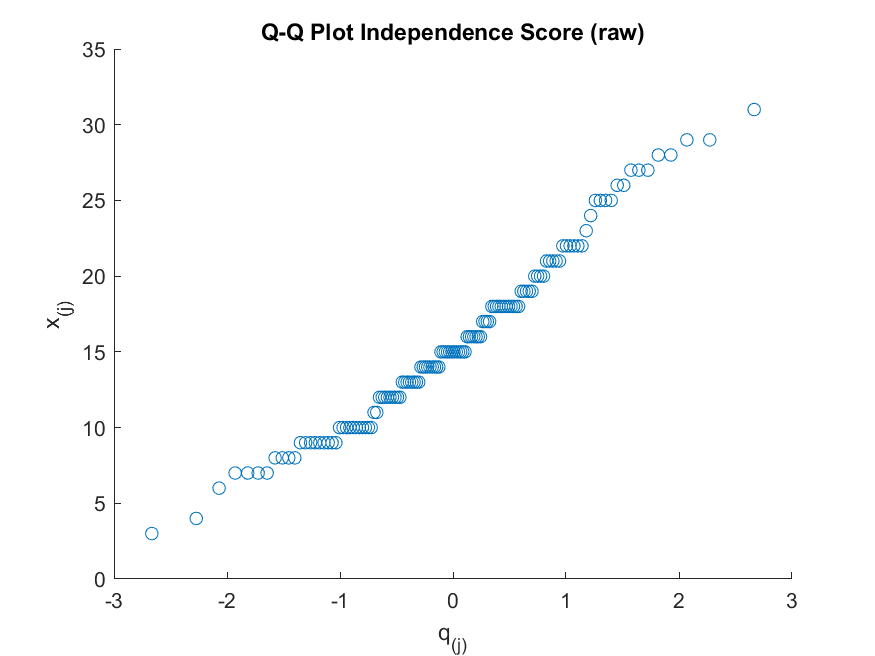
\includegraphics[scale=0.6]{./matlab/chapter-4/sol4.39.qq.1.png}
        \end{figure}
    \end{center}

    For ($x_{2}$), we're looking at the support score for 130 valid observations.
    The simulated 0.01, 0.05, and 0.10 level critical correlation coefficient test values for a sample size of 76 are, 0.9860, 0.9900, and 0.9916, respectively.
    The Q-Q correlation coefficient using the raw data is 0.9893, which is larger than the 0.01-level critical point, but not the 0.05 and 0.10, and so would be considered normal at the 0.01-level but not the 0.05 and 0.10. 
    The Q-Q plot for the raw data is below. There is some slight curvature, but a transformation also might help.

    \begin{center}
        \begin{figure}[H]
            \centering
            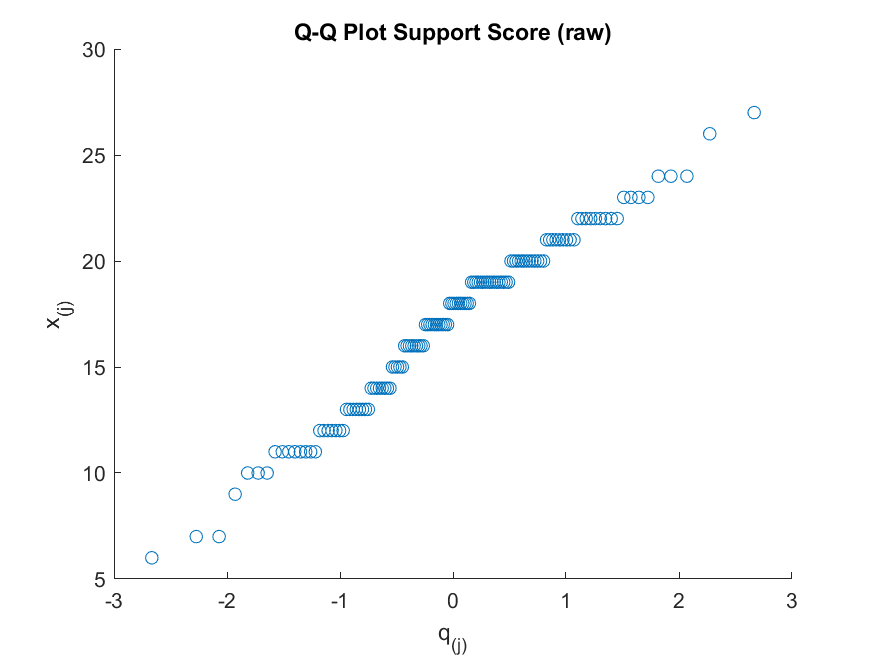
\includegraphics[scale=0.6]{./matlab/chapter-4/sol4.39.qq.2.png}
        \end{figure}
    \end{center}

    For ($x_{3}$), we're looking at the benevolence score for 130 valid observations.
    The simulated 0.01, 0.05, and 0.10 level critical correlation coefficient test values for a sample size of 76 are, 0.9860, 0.9900, and 0.9916, respectively.
    The Q-Q correlation coefficient using the raw data is 0.9925, which is larger than all three critical points, so the benevolence score would be considered normal at the 0.01, 0.05, and 0.10 levels. 
    The Q-Q plot for the raw data is below.
    There are five observations with the same score value of 29 causing a right tail effect, but overall $x_{3}$ looks marginally normal.

    \begin{center}
        \begin{figure}[H]
            \centering
            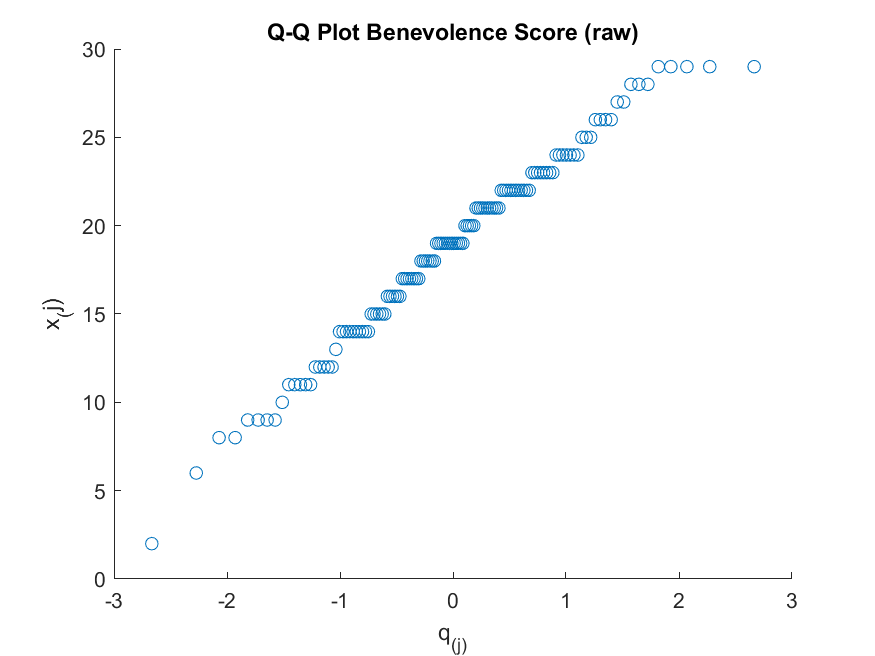
\includegraphics[scale=0.6]{./matlab/chapter-4/sol4.39.qq.3.png}
        \end{figure}
    \end{center}

    For ($x_{4}$), we're looking at the conformity score for 130 valid observations.
    The simulated 0.01, 0.05, and 0.10 level critical correlation coefficient test values for a sample size of 76 are, 0.9860, 0.9900, and 0.9916, respectively.
    The Q-Q correlation coefficient using the raw data is 0.9934, which is larger than all three critical points, so the conformity score would be considered normal at the 0.01, 0.05, and 0.10 levels. 
    The Q-Q plot for the raw data is below.
    There are three observations with the same score value of 27 causing a right tail effect, similar to $x_{3}$, but overall $x_{4}$ looks marginally normal.

    \begin{center}
        \begin{figure}[H]
            \centering
            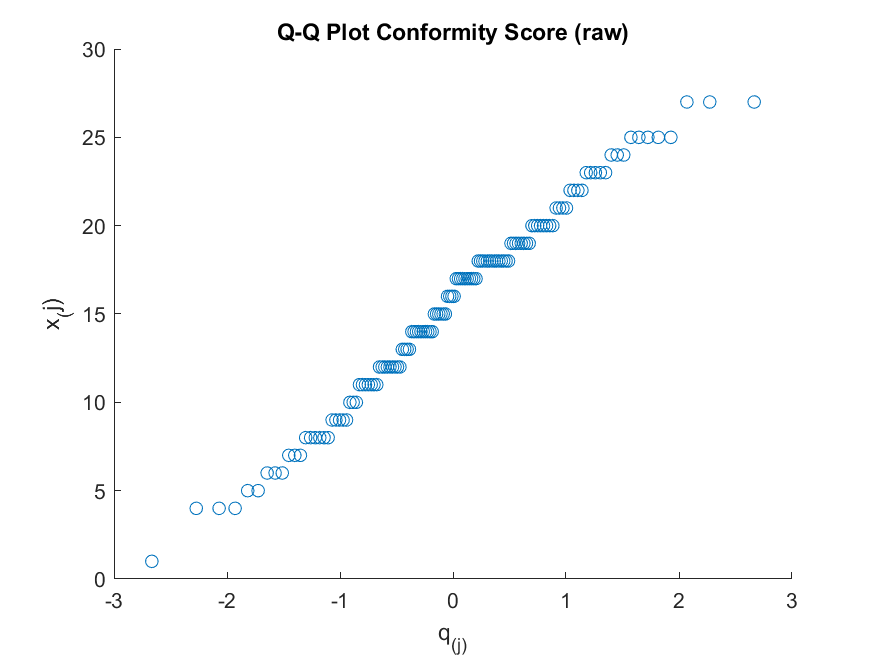
\includegraphics[scale=0.6]{./matlab/chapter-4/sol4.39.qq.4.png}
        \end{figure}
    \end{center}

    For ($x_{5}$), we're looking at the leadership score for 130 valid observations.
    The simulated 0.01, 0.05, and 0.10 level critical correlation coefficient test values for a sample size of 76 are, 0.9860, 0.9900, and 0.9916, respectively.
    The Q-Q correlation coefficient using the raw data is 0.9813, which is smaller than all three critical values, and so would not be considered normal at the 0.01, 0.05, or 0.10 levels. 
    The Q-Q plot for the raw data is below. There is curvature in the plot. A transformation would absolutely help.

    \begin{center}
        \begin{figure}[H]
            \centering
            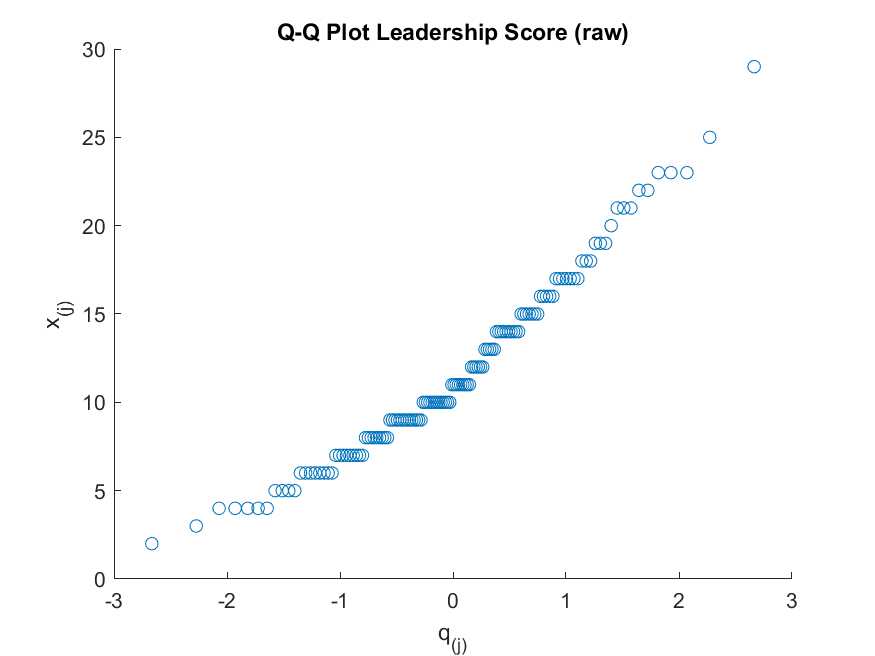
\includegraphics[scale=0.6]{./matlab/chapter-4/sol4.39.qq.5.png}
        \end{figure}
    \end{center}

    \item Using all five variables, check for multivariate normality.
    
    The $\chi^2$ plot for the five covariates is below. It looks fairly linear. However, there are three observations with large $d^{2}$ values that stand out as possible outliers.
    
    \begin{center}
        \begin{figure}[H]
            \centering
            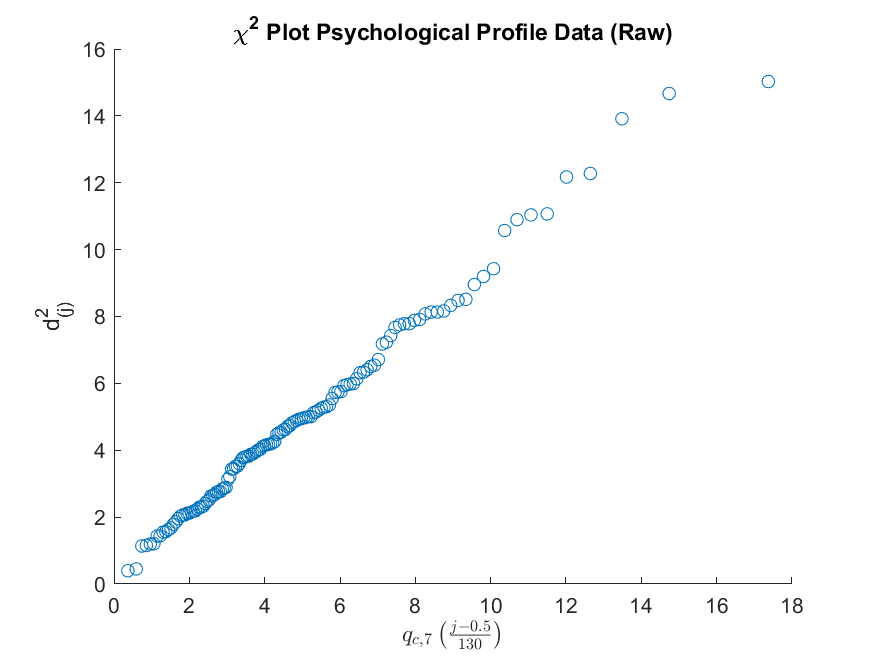
\includegraphics[scale=0.6]{./matlab/chapter-4/sol4.39.b.png}
        \end{figure}
    \end{center}

    \item Refer to part (a). For those variables that are nonnormal, determine the transformation that makes them more nearly normal.
    
    From part (a) we found that independence ($x_{1}$), support ($x_{2}$) and leadership ($x_{5}$) could use a transformation.

    For independence score, $x_{1}$, the optimal Box-Cox power transformation value found was 0.5311.
    I rounded that to 0.5, so $x_{1}^{\prime} = \sqrt{x_{1}}$. This transformation increased the Q-Q correlation coefficient to 0.9949, which is larger than the critical point values of 0.9860, 0.9900, and 0.9916 who represent the 0.01, 0.05, and 0.10 levels, respectively.
    Because of this the data would be considered normally distributed at all the usual levels.
    Below are the results of the power transformation and the Q-Q plots of the transformed data.
    The original plot shows an outlier separated out. The Q-Q plot of the transformed data was able to make the data appear more linear.

    \begin{center}
        \begin{figure}[H]
            \centering
            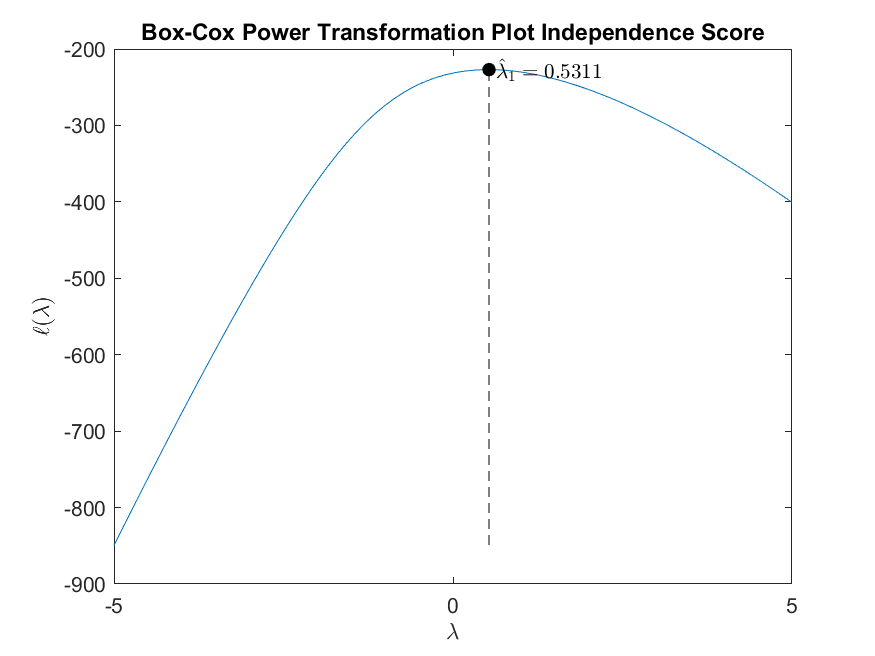
\includegraphics[scale=0.4]{./matlab/chapter-4/sol4.39.power.1.png}
        \end{figure}
    \end{center}
    
    \begin{center}
        \begin{figure}[H]
            \centering
            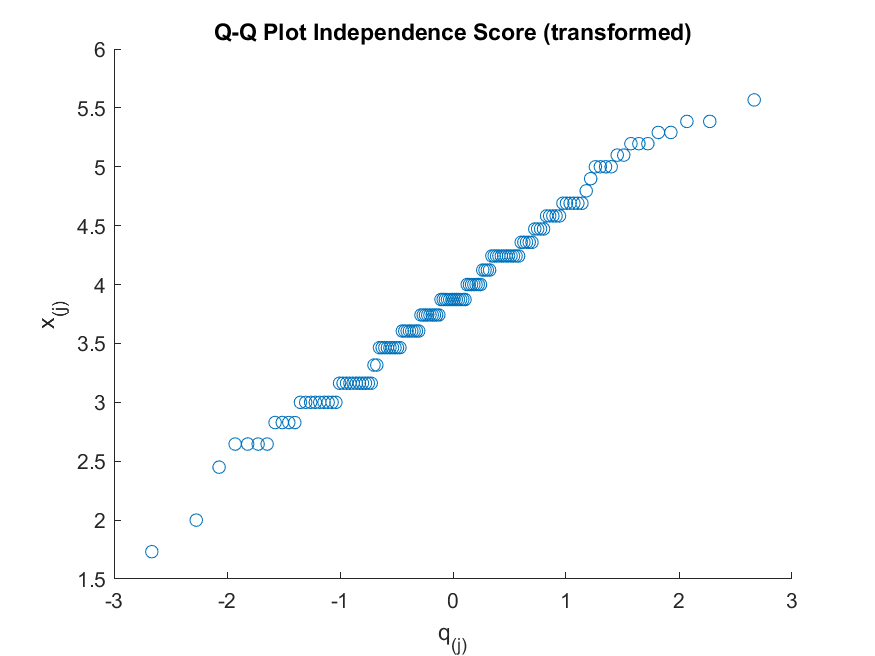
\includegraphics[scale=0.4]{./matlab/chapter-4/sol4.39.qq.tr.1.png}
        \end{figure}
    \end{center}

    For support score, $x_{2}$, the optimal Box-Cox power transformation value found was 1.3928.
    I rounded that to 1.4, so $x_{2}^{\prime} = x_{2}^{1.4}$. This transformation increased the Q-Q correlation coefficient to 0.9920, which is larger than the critical point values of 0.9860, 0.9900, and 0.9916 who represent the 0.01, 0.05, and 0.10 levels, respectively.
    Because of this the data would be considered normally distributed at all the usual levels.
    Below are the results of the power transformation and the Q-Q plots of the transformed data.
    The original plot shows an outlier separated out. The Q-Q plot of the transformed data was able to make the data appear more linear.

    \begin{center}
        \begin{figure}[H]
            \centering
            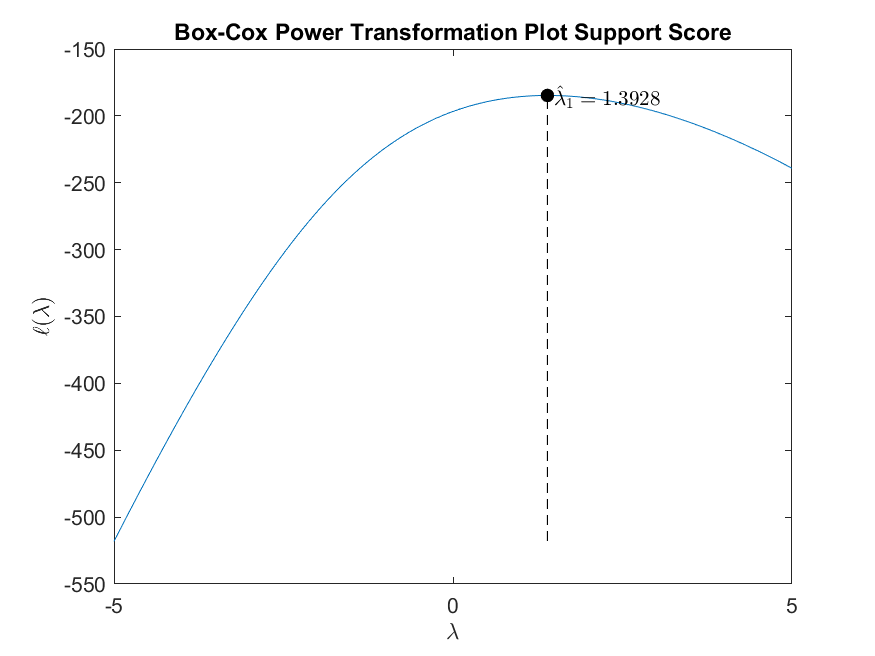
\includegraphics[scale=0.4]{./matlab/chapter-4/sol4.39.power.2.png}
        \end{figure}
    \end{center}
    
    \begin{center}
        \begin{figure}[H]
            \centering
            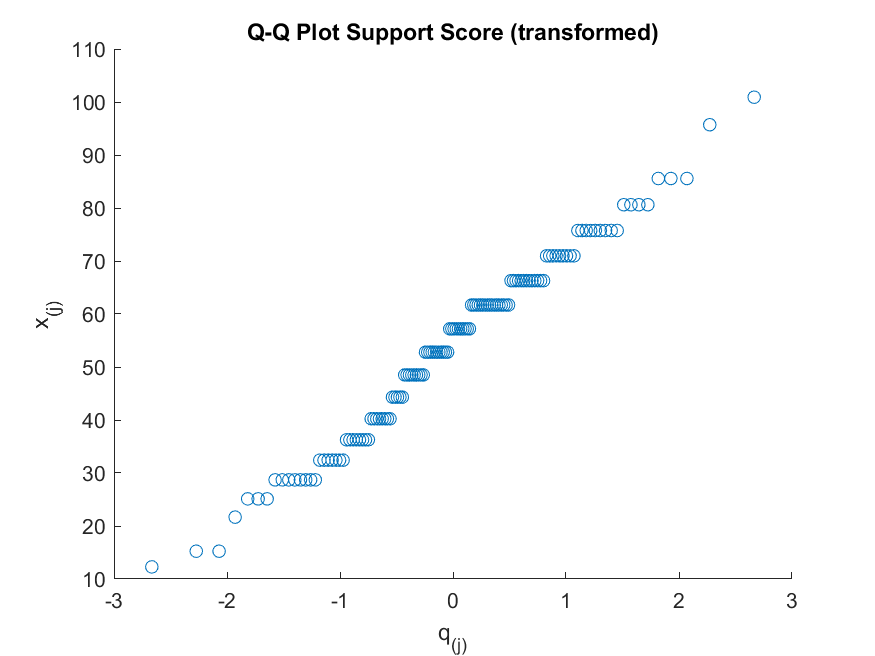
\includegraphics[scale=0.4]{./matlab/chapter-4/sol4.39.qq.tr.2.png}
        \end{figure}
    \end{center}

    For leadership score, $x_{5}$, the optimal Box-Cox power transformation value found was 0.3908.
    I rounded that to 0.4, so $x_{5}^{\prime} = x_{5}^{0.4}$. This transformation increased the Q-Q correlation coefficient to 0.9965, which is larger than the critical point values of 0.9860, 0.9900, and 0.9916 who represent the 0.01, 0.05, and 0.10 levels, respectively.
    Because of this the data would be considered normally distributed at all the usual levels.
    Below are the results of the power transformation and the Q-Q plots of the transformed data.
    The original plot shows an outlier separated out. The Q-Q plot of the transformed data was able to make the data appear more linear.

    \begin{center}
        \begin{figure}[H]
            \centering
            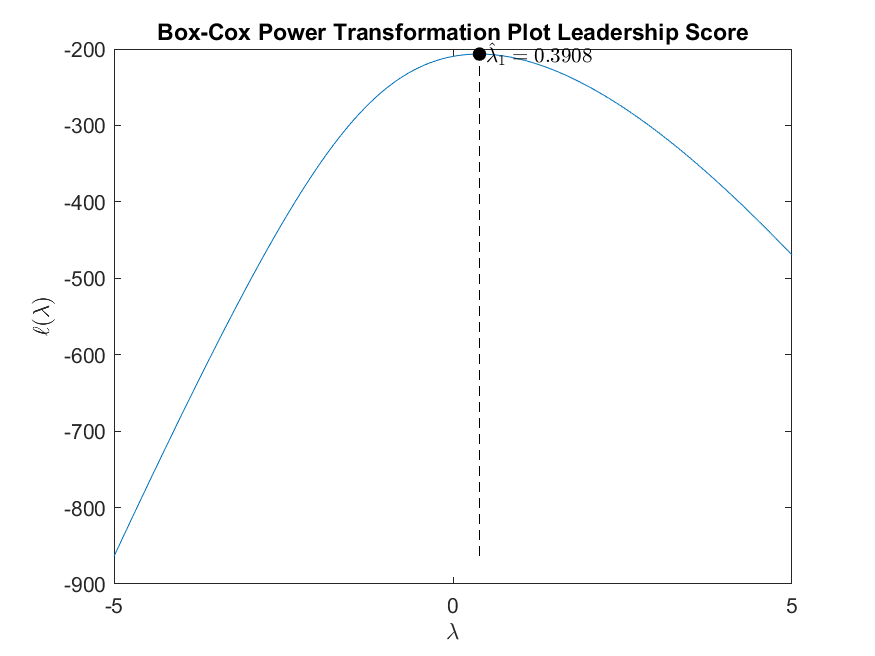
\includegraphics[scale=0.4]{./matlab/chapter-4/sol4.39.power.5.png}
        \end{figure}
    \end{center}
    
    \begin{center}
        \begin{figure}[H]
            \centering
            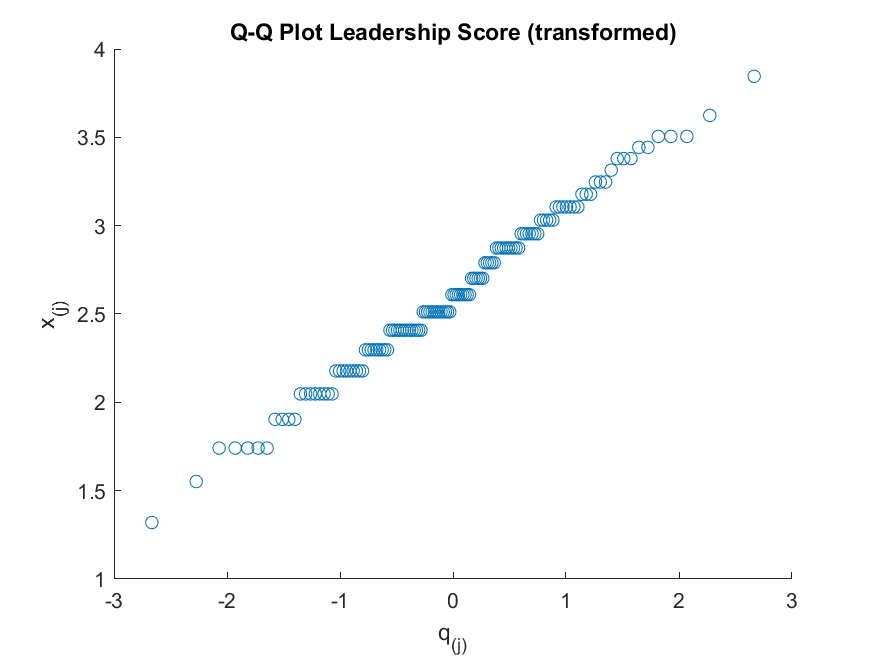
\includegraphics[scale=0.4]{./matlab/chapter-4/sol4.39.qq.tr.5.png}
        \end{figure}
    \end{center}

\end{enumerate}